\chapter{METODOLOGI PENELITIAN}

Bab ini menjelaskan metode yang digunakan dalam penelitian. Berbeda dengan
Bab 2 yang membahas teori dan penelitian terdahulu, Bab 3 berfokus pada
bagaimana penelitian dilakukan oleh penulis.

Bagian ini menjelaskan proses penelitian secara sistematis mulai dari
rancangan penelitian, dataset yang digunakan, metode yang diterapkan,
hingga proses evaluasi hasil penelitian.

%%%%%%%%%%%%%%%%%%%%%%%%%%%%%%%%%%%%%%%%%%%%%%%%%%
\section{Metodologi Penelitian}
%%%%%%%%%%%%%%%%%%%%%%%%%%%%%%%%%%%%%%%%%%%%%%%%%%

Bagian ini menjelaskan pendekatan penelitian yang digunakan. Metodologi
dapat berupa pendekatan eksperimental, studi kasus, simulasi, atau
pendekatan lainnya yang sesuai dengan tujuan penelitian.

Penulis juga perlu menjelaskan alasan pemilihan metode tersebut serta
bagaimana metode tersebut digunakan untuk menjawab rumusan masalah
yang telah dijelaskan pada Bab 1.

%%%%%%%%%%%%%%%%%%%%%%%%%%%%%%%%%%%%%%%%%%%%%%%%%%
\section{Tahapan Penelitian}
%%%%%%%%%%%%%%%%%%%%%%%%%%%%%%%%%%%%%%%%%%%%%%%%%%

Tahapan penelitian menjelaskan alur proses penelitian dari awal hingga
akhir secara sistematis.

\textbf{Contoh} alur penelitian biasanya dapat ditampilkan dalam bentuk diagram seperti pada Gambar \ref{fig:research-flow}.

\begin{figure}[H]
\centering
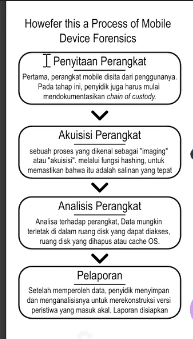
\includegraphics[width=0.8\textwidth]{images/contoh-flow.png}
\caption{Alur tahapan penelitian}
\label{fig:research-flow}
\end{figure}

Berdasarkan Gambar \ref{fig:research-flow}, tahapan penelitian terdiri dari:

\begin{enumerate}
\item Studi literatur
\item Pengumpulan dataset
\item Perancangan metode
\item Implementasi sistem
\item Evaluasi performa
\end{enumerate}

%%%%%%%%%%%%%%%%%%%%%%%%%%%%%%%%%%%%%%%%%%%%%%%%%%
\section{Dataset Penelitian}
%%%%%%%%%%%%%%%%%%%%%%%%%%%%%%%%%%%%%%%%%%%%%%%%%%

Bagian ini menjelaskan dataset yang digunakan dalam penelitian. Penjelasan
meliputi sumber dataset, jumlah data, fitur yang digunakan, serta proses
preprocessing yang dilakukan.

\subsection{Sumber Dataset}

Dataset yang digunakan dalam penelitian ini berasal dari sumber terbuka
atau repository penelitian yang relevan.

\subsection{Preprocessing Data}

Tahapan preprocessing dilakukan untuk membersihkan dan menyiapkan data
sebelum digunakan dalam proses penelitian.

%%%%%%%%%%%%%%%%%%%%%%%%%%%%%%%%%%%%%%%%%%%%%%%%%%
\section{Metode Penelitian}
%%%%%%%%%%%%%%%%%%%%%%%%%%%%%%%%%%%%%%%%%%%%%%%%%%

Bagian ini menjelaskan metode atau algoritma yang digunakan dalam penelitian.
Penjelasan harus mencakup cara kerja metode, parameter yang digunakan,
serta bagaimana metode tersebut diterapkan pada dataset.

\subsection{Arsitektur Sistem}

Arsitektur sistem menggambarkan hubungan antara komponen yang digunakan
dalam penelitian.

\subsection{Algoritma yang Digunakan}

Bagian ini menjelaskan algoritma atau model yang digunakan dalam penelitian.

%%%%%%%%%%%%%%%%%%%%%%%%%%%%%%%%%%%%%%%%%%%%%%%%%%
\section{Evaluasi dan Pengukuran Kinerja}
%%%%%%%%%%%%%%%%%%%%%%%%%%%%%%%%%%%%%%%%%%%%%%%%%%

Bagian ini menjelaskan metode evaluasi yang digunakan untuk mengukur
kinerja sistem yang dikembangkan.

Contoh metrik evaluasi yang sering digunakan antara lain:

\begin{itemize}
\item Accuracy
\item Precision
\item Recall
\item F1-score
\end{itemize}

%%%%%%%%%%%%%%%%%%%%%%%%%%%%%%%%%%%%%%%%%%%%%%%%%%
\section{Implementasi Sistem}
%%%%%%%%%%%%%%%%%%%%%%%%%%%%%%%%%%%%%%%%%%%%%%%%%%

Bagian ini menjelaskan lingkungan implementasi penelitian seperti
perangkat keras, perangkat lunak, serta framework yang digunakan.

%%%%%%%%%%%%%%%%%%%%%%%%%%%%%%%%%%%%%%%%%%%%%%%%%%
\section{Pedoman Penggunaan Sitasi dan BibTeX}
%%%%%%%%%%%%%%%%%%%%%%%%%%%%%%%%%%%%%%%%%%%%%%%%%%

Pada template ini, pengelolaan referensi dilakukan menggunakan sistem
BibTeX melalui file \texttt{references.bib}. Semua referensi yang digunakan
dalam penelitian harus disimpan dalam file tersebut.

\subsection{Menambahkan Referensi ke references.bib}

Langkah-langkah menambahkan referensi adalah sebagai berikut:

\begin{enumerate}

\item Setelah mendapatkan judul artikel yang ingin disitasi, salin judul tersebut dan cari melalui Google Scholar seperti pada Gambar \ref{fig:scholar-search}.

\begin{figure}[H]
\centering

\includegraphics[width=0.8\textwidth]{images/Cite1.png}
\caption{Alur tahapan penelitian}
\label{fig:scholar-search}
\end{figure}

\item Setelah menemukan artikel yang dimaksud, pada hasil pencarian akan terdapat tombol \textit{Cite} atau \textit{Kutip} seperti pada Gambar \ref{fig:scholar-found}.

\begin{figure}[H]
\centering
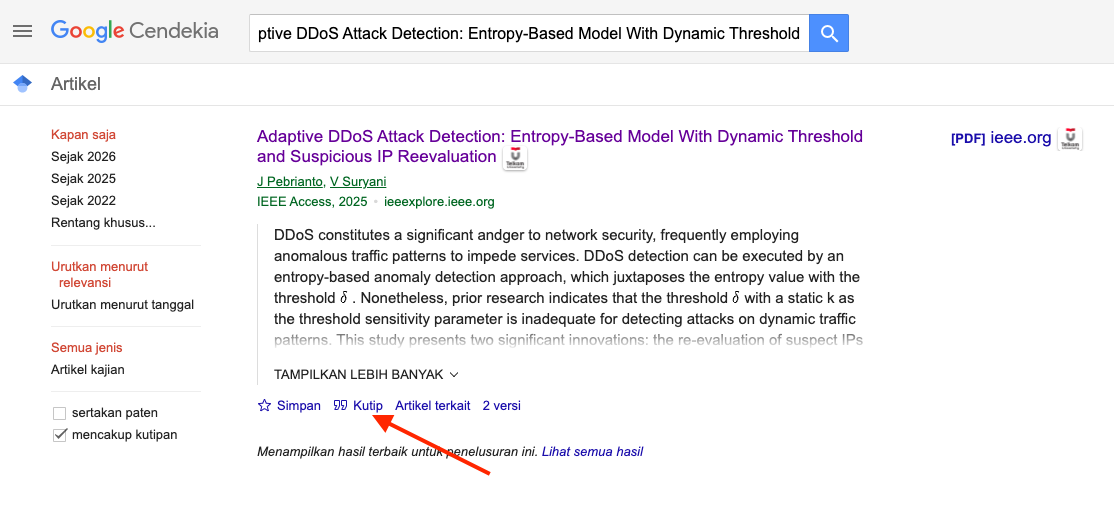
\includegraphics[width=0.8\textwidth]{images/Cite3.png}
\caption{Alur tahapan penelitian}
\label{fig:scholar-found}
\end{figure}

\item Klik tombol tersebut sehingga akan muncul beberapa format sitasi seperti pada Gambar \ref{fig:scholar-cite}.

\begin{figure}[H]
\centering
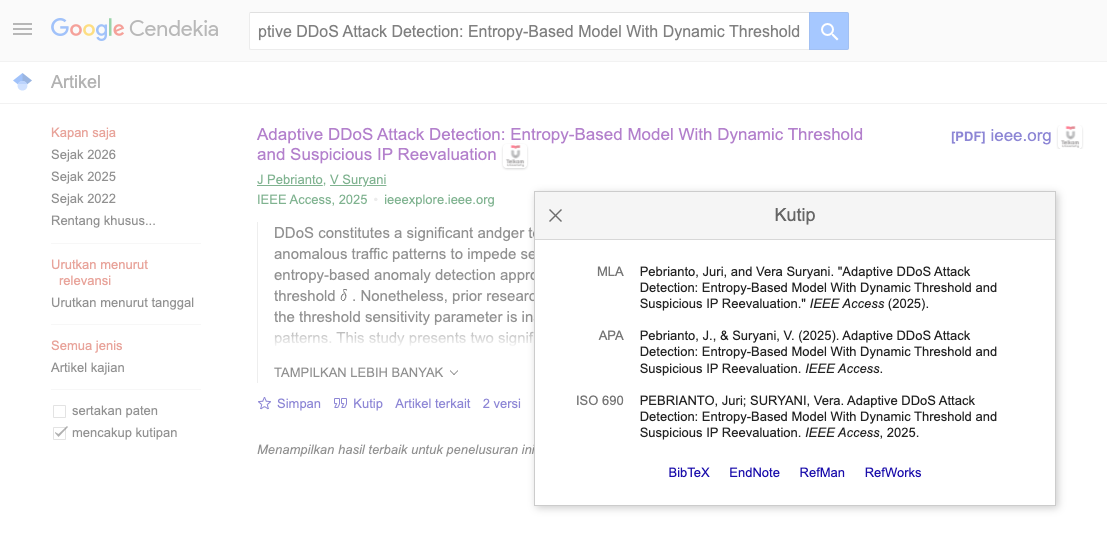
\includegraphics[width=0.8\textwidth]{images/Cite4.png}
\caption{Alur tahapan penelitian}
\label{fig:scholar-cite}
\end{figure}

\item Pilih format \textbf{BibTeX}, kemudian salin seluruh skrip BibTeX yang ditampilkan seperti pada Gambar \ref{fig:scholar-bib}.

\begin{figure}[H]
\centering
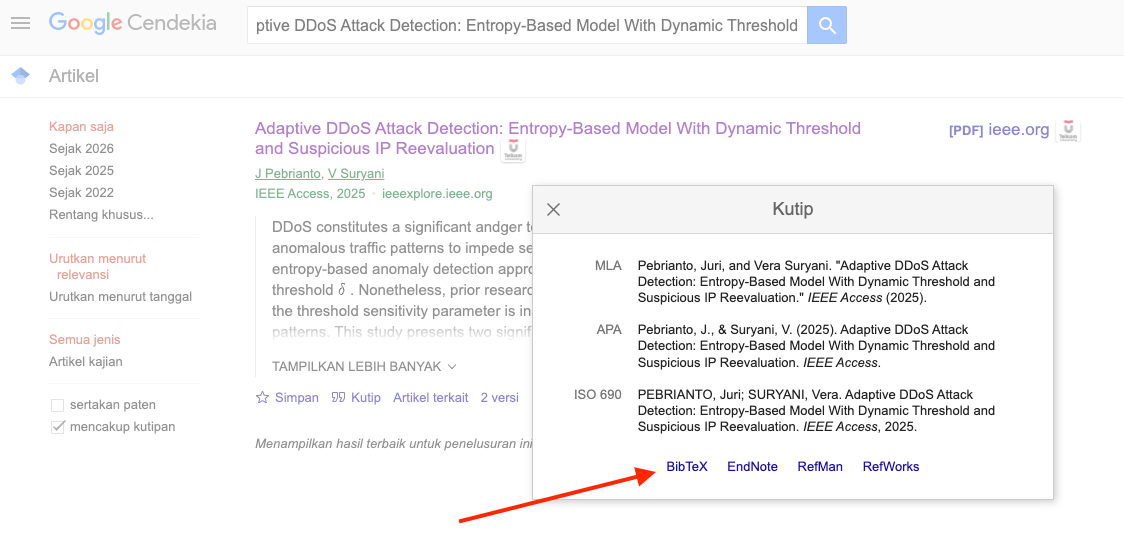
\includegraphics[width=0.8\textwidth]{images/Cite5.png}
\caption{Alur tahapan penelitian}
\label{fig:scholar-bib}
\end{figure}

\item Tempelkan skrip tersebut pada file \texttt{references.bib} yang
terdapat pada project \LaTeX.
\end{enumerate}

Contoh skrip BibTeX yang dimasukkan ke dalam file \texttt{references.bib}:

\begin{verbatim}
@article{pebrianto2025adaptive,
  title={Adaptive DDoS Attack Detection: Entropy-Based Model With Dynamic Threshold and Suspicious IP Reevaluation},
  author={Pebrianto, Juri and Suryani, Vera},
  journal={IEEE Access},
  year={2025},
  publisher={IEEE}
}
\end{verbatim}

%%%%%%%%%%%%%%%%%%%%%%%%%%%%%%%%%%%%%%%%%%%%%%%%%%
\subsection{Cara Menggunakan Sitasi}
%%%%%%%%%%%%%%%%%%%%%%%%%%%%%%%%%%%%%%%%%%%%%%%%%%

Setelah referensi ditambahkan ke file \texttt{references.bib}, referensi
tersebut dapat dipanggil dalam dokumen menggunakan perintah sitasi.

Contoh penggunaan:

\begin{itemize}

\item Menggunakan \texttt{\textbackslash cite}

\begin{verbatim}
\cite{pebrianto2025adaptive}
\end{verbatim}

Akan menghasilkan sitasi seperti:

Pebrianto dan Suryani (2025)

\item Menggunakan \texttt{\textbackslash parencite}

\begin{verbatim}
\parencite{pebrianto2025adaptive}
\end{verbatim}

Akan menghasilkan sitasi seperti:

(Pebrianto dan Suryani, 2025)

\end{itemize}

%%%%%%%%%%%%%%%%%%%%%%%%%%%%%%%%%%%%%%%%%%%%%%%%%%
\subsection{Daftar Pustaka Otomatis}
%%%%%%%%%%%%%%%%%%%%%%%%%%%%%%%%%%%%%%%%%%%%%%%%%%

Semua referensi yang dipanggil menggunakan perintah sitasi akan secara
otomatis muncul pada bagian daftar pustaka.

Oleh karena itu, pastikan setiap referensi yang digunakan telah ditambahkan
ke dalam file \texttt{references.bib}.